\section{Réalisation et implémentation}

J'ai choisi de ne pas présenter l'implémentation faite partie par partie, mais de présenter l'implémentation finale car elle contient les éléments correspondant à chacune des parties. 

\subsection{Création de l'IP axi lite}

Une base de code nous était fournie dans ce laboratoire. J'ai commenté le code afin d'expliquer son fonctionnement, j'ai mis en annexe le résultat obtenu. Dans la partie simulation, nous parlerons des tests effectués avec vsim, mais ici je n'ai pas grand-chose à ajouter, le code ayant été commenté dans son entier.

\subsection{Ajout de l'IP dans Qsys}
Certaines informations nous étaient fournies dans cette partie. J'ai donc respecté les consignes données, tout en rajoutant certaines choses :\\
\begin{itemize}
	\item Ajout du composant dans QSys
	\item Ajout du fichier vhdl correspondant à l'IP dans le nouveau composant
	\item Appui sur le bouton "Analyze Synthesis Files" afin de récupérer les signaux
	\item Ajout des interfaces (altera\_axi4lite\_slave,clock\_sink,conduit\_end,interrupt\_sender,reset\_sink)
	\item Assignation et configuration des signaux de l'IP aux interfaces\\
\end{itemize}
Le résultat final dans l'onglet "Signals \& Interfaces" est le suivant : \\
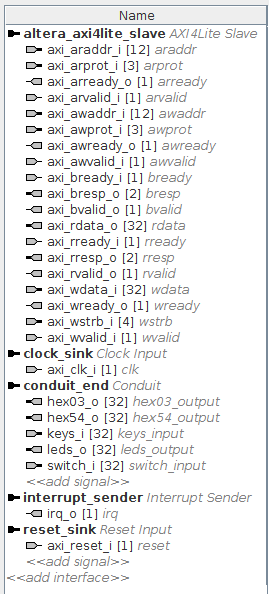
\includegraphics[scale=0.6]{./images/axilite_ip_signals_interface.png}
\captionof{figure}{Laboratoire 5 : Signals et Interfaces}

\subsection{Actions dans le projet Qsys}
Comme dans le laboratoire 2, certaines actions devaient être effectuées dans Qsys afin de permettre le fonctionnement du programme : \\

\begin{itemize}
	\item Il faut activer dans la configuration de hps\_0 , sous "Fpga inteface" -> "interrupts", l'option "Enable FPGA-to-HPS interrupts"
	\item L'IP qui doit bénéficier des interruptions doit être linké sur l'un des deux champs "f2h\_irq0/1".
	\item Dans la colonne IRQ aussi, l'interruption de l'interrupt sender de l'IP doit être linkée sur l'un des deux champs vu plus haut. Dans notre cas, l'interruption porte le numéro 0 et est linkée sur "f2h\_irq0", ce qui implique que le numéro de l'interruption sera le numéro 0 de la fpga(numéro d'interruption 72)
	\item Les autres interfaces de l'IP doivent être câblé sur les bons éléments dans le projet Qsys comme le présente l'image ci-dessous. \\
\end{itemize}
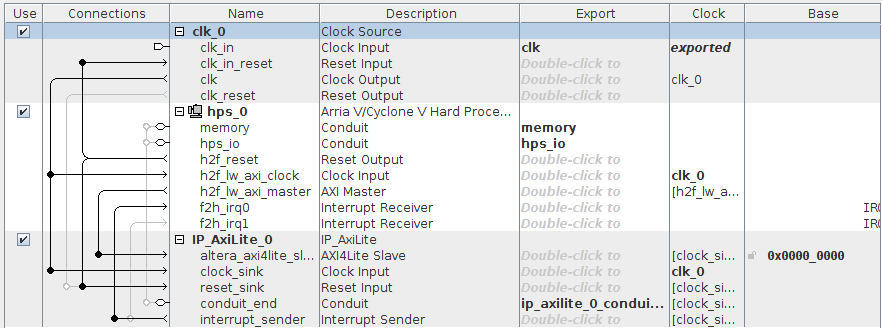
\includegraphics[scale=0.5]{./images/cablage_qsys.png}
\captionof{figure}{Laboratoire 5 : Projet Qsys}

Comme on peut le voir, l'interface Axilite est câblé sur le bus h2f\_lw\_axi\_master avec comme base 0x00000000, ce qui veut dire que l'adresse de base à laquelle il faut ajouter les offsets du plan d'adressage sera l'adresse du début du bus h2f\_lw, soit 0xFF200000. 
\subsection{Implémentation dans le fichier top du projet}
Après avoir généré le code VHDL du projet Qsys, je devais ajouter le composant au fichier top du projet Quartus. J'ai copié le résultat obtenu avec Qsys pour l'attribution des sorties et entrées du composant crée, et j'ai dû ajouter des traitements supplémentaires, voici lesdites modifications : \\
\begin{lstlisting}[language=VHDL]
 ...
 
	signal temp_hex03_s : std_logic_vector(31 downto 0);
	signal temp_hex45_s : std_logic_vector(31 downto 0);
	signal temp_leds_s : std_logic_vector(31 downto 0);
	signal temp_key : std_logic_vector(31 downto 0);
	signal temp_sw  : std_logic_vector(31 downto 0);
	signal temp_zero_key : std_logic_vector(31-4 downto 0);
	signal temp_zero_sw  : std_logic_vector(31-10 downto 0);

begin

	---------------------------------------------------------
	--  HPS mapping
	---------------------------------------------------------
	temp_zero_key <= (others => '0');
	temp_zero_sw <= (others => '0');
	temp_key <=  temp_zero_key & KEY_i ;
	temp_sw <= temp_zero_sw & SW_i;

	System : component qsys_system
	...
	 -- User input-output
	ip_axilite_0_conduit_end_hex03_output : out   std_logic_vector(31 downto 0);                    -- hex03_output
	ip_axilite_0_conduit_end_hex54_output : out   std_logic_vector(31 downto 0);                    -- hex54_output
	ip_axilite_0_conduit_end_keys_input   : in    std_logic_vector(31 downto 0) := (others => 'X'); -- keys_input
	ip_axilite_0_conduit_end_leds_output  : out   std_logic_vector(31 downto 0);                    -- leds_output
	ip_axilite_0_conduit_end_switch_input : in    std_logic_vector(31 downto 0) := (others => 'X'); -- switch_input
	...
	);

	HEX0_o <= temp_hex03_s(6 downto 0);
	HEX1_o <= temp_hex03_s(14 downto 8);
	HEX2_o <= temp_hex03_s(22 downto 16);
	HEX3_o <= temp_hex03_s(30 downto 24);
	HEX4_o <= temp_hex45_s(6 downto 0);
	HEX5_o <= temp_hex45_s(14 downto 8);
	LEDR_o <= temp_leds_s(9 downto 0);
end top;

\end{lstlisting}

Le premier traitement, celui concernant les keys et les switchs, permet de formater les inputs des keys et des switchs reçus afin de nous assurer que le plan d'adressage soit respecté et que les bits devant être lu comme '0' le soit bien. Le traitement concernant les afficheurs 7 segments et les leds permet de réduire la taille des valeurs reçues depuis le composant afin de pouvoir les adapter à la taille des sorties.

\subsection{Code C}
Le code C ressemble beaucoup au code C du laboratoire précédent, le laboratoire 2. La seule différence résidant au final dans la gestion de deux afficheurs 7 segments en plus, mais la méthode utilisée reste la même. J'ai tout de même modifié légèrement le code afin de réduire le nombre de lectures effectuées, suite aux remarques concernant le laboratoire précédent. Le code C peut être trouvé dans le projet, je ne vais pas plus en parler ici, la gestion des interruptions se fait de la même manière. Les adresses utilisées ont dû être légèrement modifiée afin de coller avec le plan d'adressage.
